% Options for packages loaded elsewhere
\PassOptionsToPackage{unicode}{hyperref}
\PassOptionsToPackage{hyphens}{url}
%
\documentclass[
]{book}
\usepackage{lmodern}
\usepackage{amssymb,amsmath}
\usepackage{ifxetex,ifluatex}
\ifnum 0\ifxetex 1\fi\ifluatex 1\fi=0 % if pdftex
  \usepackage[T1]{fontenc}
  \usepackage[utf8]{inputenc}
  \usepackage{textcomp} % provide euro and other symbols
\else % if luatex or xetex
  \usepackage{unicode-math}
  \defaultfontfeatures{Scale=MatchLowercase}
  \defaultfontfeatures[\rmfamily]{Ligatures=TeX,Scale=1}
\fi
% Use upquote if available, for straight quotes in verbatim environments
\IfFileExists{upquote.sty}{\usepackage{upquote}}{}
\IfFileExists{microtype.sty}{% use microtype if available
  \usepackage[]{microtype}
  \UseMicrotypeSet[protrusion]{basicmath} % disable protrusion for tt fonts
}{}
\makeatletter
\@ifundefined{KOMAClassName}{% if non-KOMA class
  \IfFileExists{parskip.sty}{%
    \usepackage{parskip}
  }{% else
    \setlength{\parindent}{0pt}
    \setlength{\parskip}{6pt plus 2pt minus 1pt}}
}{% if KOMA class
  \KOMAoptions{parskip=half}}
\makeatother
\usepackage{xcolor}
\IfFileExists{xurl.sty}{\usepackage{xurl}}{} % add URL line breaks if available
\IfFileExists{bookmark.sty}{\usepackage{bookmark}}{\usepackage{hyperref}}
\hypersetup{
  pdftitle={Thermodynamics One},
  pdfauthor={marcus ashford, phd},
  hidelinks,
  pdfcreator={LaTeX via pandoc}}
\urlstyle{same} % disable monospaced font for URLs
\usepackage{color}
\usepackage{fancyvrb}
\newcommand{\VerbBar}{|}
\newcommand{\VERB}{\Verb[commandchars=\\\{\}]}
\DefineVerbatimEnvironment{Highlighting}{Verbatim}{commandchars=\\\{\}}
% Add ',fontsize=\small' for more characters per line
\usepackage{framed}
\definecolor{shadecolor}{RGB}{248,248,248}
\newenvironment{Shaded}{\begin{snugshade}}{\end{snugshade}}
\newcommand{\AlertTok}[1]{\textcolor[rgb]{0.94,0.16,0.16}{#1}}
\newcommand{\AnnotationTok}[1]{\textcolor[rgb]{0.56,0.35,0.01}{\textbf{\textit{#1}}}}
\newcommand{\AttributeTok}[1]{\textcolor[rgb]{0.77,0.63,0.00}{#1}}
\newcommand{\BaseNTok}[1]{\textcolor[rgb]{0.00,0.00,0.81}{#1}}
\newcommand{\BuiltInTok}[1]{#1}
\newcommand{\CharTok}[1]{\textcolor[rgb]{0.31,0.60,0.02}{#1}}
\newcommand{\CommentTok}[1]{\textcolor[rgb]{0.56,0.35,0.01}{\textit{#1}}}
\newcommand{\CommentVarTok}[1]{\textcolor[rgb]{0.56,0.35,0.01}{\textbf{\textit{#1}}}}
\newcommand{\ConstantTok}[1]{\textcolor[rgb]{0.00,0.00,0.00}{#1}}
\newcommand{\ControlFlowTok}[1]{\textcolor[rgb]{0.13,0.29,0.53}{\textbf{#1}}}
\newcommand{\DataTypeTok}[1]{\textcolor[rgb]{0.13,0.29,0.53}{#1}}
\newcommand{\DecValTok}[1]{\textcolor[rgb]{0.00,0.00,0.81}{#1}}
\newcommand{\DocumentationTok}[1]{\textcolor[rgb]{0.56,0.35,0.01}{\textbf{\textit{#1}}}}
\newcommand{\ErrorTok}[1]{\textcolor[rgb]{0.64,0.00,0.00}{\textbf{#1}}}
\newcommand{\ExtensionTok}[1]{#1}
\newcommand{\FloatTok}[1]{\textcolor[rgb]{0.00,0.00,0.81}{#1}}
\newcommand{\FunctionTok}[1]{\textcolor[rgb]{0.00,0.00,0.00}{#1}}
\newcommand{\ImportTok}[1]{#1}
\newcommand{\InformationTok}[1]{\textcolor[rgb]{0.56,0.35,0.01}{\textbf{\textit{#1}}}}
\newcommand{\KeywordTok}[1]{\textcolor[rgb]{0.13,0.29,0.53}{\textbf{#1}}}
\newcommand{\NormalTok}[1]{#1}
\newcommand{\OperatorTok}[1]{\textcolor[rgb]{0.81,0.36,0.00}{\textbf{#1}}}
\newcommand{\OtherTok}[1]{\textcolor[rgb]{0.56,0.35,0.01}{#1}}
\newcommand{\PreprocessorTok}[1]{\textcolor[rgb]{0.56,0.35,0.01}{\textit{#1}}}
\newcommand{\RegionMarkerTok}[1]{#1}
\newcommand{\SpecialCharTok}[1]{\textcolor[rgb]{0.00,0.00,0.00}{#1}}
\newcommand{\SpecialStringTok}[1]{\textcolor[rgb]{0.31,0.60,0.02}{#1}}
\newcommand{\StringTok}[1]{\textcolor[rgb]{0.31,0.60,0.02}{#1}}
\newcommand{\VariableTok}[1]{\textcolor[rgb]{0.00,0.00,0.00}{#1}}
\newcommand{\VerbatimStringTok}[1]{\textcolor[rgb]{0.31,0.60,0.02}{#1}}
\newcommand{\WarningTok}[1]{\textcolor[rgb]{0.56,0.35,0.01}{\textbf{\textit{#1}}}}
\usepackage{longtable,booktabs}
% Correct order of tables after \paragraph or \subparagraph
\usepackage{etoolbox}
\makeatletter
\patchcmd\longtable{\par}{\if@noskipsec\mbox{}\fi\par}{}{}
\makeatother
% Allow footnotes in longtable head/foot
\IfFileExists{footnotehyper.sty}{\usepackage{footnotehyper}}{\usepackage{footnote}}
\makesavenoteenv{longtable}
\usepackage{graphicx}
\makeatletter
\def\maxwidth{\ifdim\Gin@nat@width>\linewidth\linewidth\else\Gin@nat@width\fi}
\def\maxheight{\ifdim\Gin@nat@height>\textheight\textheight\else\Gin@nat@height\fi}
\makeatother
% Scale images if necessary, so that they will not overflow the page
% margins by default, and it is still possible to overwrite the defaults
% using explicit options in \includegraphics[width, height, ...]{}
\setkeys{Gin}{width=\maxwidth,height=\maxheight,keepaspectratio}
% Set default figure placement to htbp
\makeatletter
\def\fps@figure{htbp}
\makeatother
\setlength{\emergencystretch}{3em} % prevent overfull lines
\providecommand{\tightlist}{%
  \setlength{\itemsep}{0pt}\setlength{\parskip}{0pt}}
\setcounter{secnumdepth}{5}
\usepackage{booktabs}

% chemical nomenclature
\usepackage[version=4,layout=stacked,arrows=pgf-filled]{mhchem}
\ifluatex
  \usepackage{selnolig}  % disable illegal ligatures
\fi
\usepackage[]{natbib}
\bibliographystyle{apalike}

\title{Thermodynamics One}
\usepackage{etoolbox}
\makeatletter
\providecommand{\subtitle}[1]{% add subtitle to \maketitle
  \apptocmd{\@title}{\par {\large #1 \par}}{}{}
}
\makeatother
\subtitle{Semester Projects}
\author{marcus ashford, phd}
\date{2020-10-14}

\begin{document}
\maketitle

{
\setcounter{tocdepth}{1}
\tableofcontents
}
\begin{equation}
x^2 - \frac{y}{4}
\end{equation}

\hypertarget{prerequisites}{%
\chapter*{Prerequisites}\label{prerequisites}}
\addcontentsline{toc}{chapter}{Prerequisites}

\hypertarget{orc}{%
\section{ORC}\label{orc}}

This is a \emph{sample} book written in \textbf{Markdown}. You can use anything that Pandoc's Markdown supports, e.g., a math equation \(a^2 + b^2 = c^2\) or \ce{H2SO4} .

The \textbf{bookdown} package can be installed from CRAN or Github:

\begin{Shaded}
\begin{Highlighting}[]
\KeywordTok{install.packages}\NormalTok{(}\StringTok{"bookdown"}\NormalTok{)}
\CommentTok{\# or the development version}
\CommentTok{\# devtools::install\_github("rstudio/bookdown")}
\end{Highlighting}
\end{Shaded}

Remember each Rmd file contains one and only one chapter, and a chapter is defined by the first-level heading \texttt{\#}.

To compile this example to PDF, you need XeLaTeX. You are recommended to install TinyTeX (which includes XeLaTeX): \url{https://yihui.org/tinytex/}.

\mainmatter

\hypertarget{stadium-roof}{%
\chapter{Stadium Roof}\label{stadium-roof}}

Estimate the hearing/cooling requirements for adding a roof to an outdoor stadium. I've described the stadium in terms of Bryant-Denny, but any stadium would do. Model the stadium as a sphere that would reasonably approximate the interior volume of your proposed structure. For reference, the Superdome encloses about 3,500,000 m3.

You have two worst case scenarios to consider.

\hypertarget{summer-day}{%
\section{Summer Day}\label{summer-day}}

Set the outside temperature to be the hottest day of the year for the stadium location. Fill it to seating capacity. This will be a standard refrigeration (air conditioning) system like in your text. You need to account for the following:

\begin{enumerate}
\def\labelenumi{\arabic{enumi}.}
\tightlist
\item
  Heat generated by the occupants\\
\item
  Heat transfer in through the roof (top hemisphere). See \#3 below.\\
\item
  solar irradiation (hottest day)\\
\item
  conduction/convection with outside\\
\item
  Adiabatic lower hemisphere
\end{enumerate}

\hypertarget{winter-night}{%
\section{Winter Night}\label{winter-night}}

Set the outside temperature to be the coldest night of the year for the stadium location. Choose natural gas heating or a heat pump with COPHP = 1 + COPR of the Summer Day AC system. Assume the following:

\begin{enumerate}
\def\labelenumi{\arabic{enumi}.}
\tightlist
\item
  No occupants\\
\item
  No solar irradiation.\\
\item
  Adiabatic lower hemisphere\\
\item
  Heat transfer out through the roof. See \#3 below.
\end{enumerate}

\hypertarget{calculations}{%
\section{Calculations}\label{calculations}}

Determine the energy required to maintain a steady comfortable indoor temperature (20 °C) for both scenarios. For context, calculate the energy cost (\$/hour). Use the local cost of energy, discounted 20\%.

Using the heating and cooling systems from (1), determine the time it takes to reach the comfort temperature when starting from an unoccupied arena at the outdoor temperature (ie, a huge volume of air).

Compare the heating cost to electric heating, which is often used in cheap apartments blocks. In electric heating, electricity is converted directly to heat ( = 100\%!).

\hypertarget{useful-information}{%
\section{Useful Information}\label{useful-information}}

A reasonable COP for an arena-scale air-conditioning system is COP = 3 - 3.5.
Solar irradiation for your location can be found in an online almanac or from NOAA or DOE. It'll be a heat flux in units of W/m2. The roof will reflect a portion of this energy. A good source for solar reflectance values (they range from 0-1) for roof coatings can be found at the Cool Roofs Ratings Council (\url{https://coolroofs.org/directory/results}). Apply this heat flux to the entire roof area.
Estimate the thermal conductivity of your roof at 0.3 W/K. Heat flux (power/area) is expressed as

\begin{align}
 q'' &= -k \frac{\text dT}{\text dx} \\
 \text{where}\hfill \notag \\
 q'' &\equiv \text{heat flux} \left[ \frac{W}{m^2} \right]  \notag \\
 k &\equiv \text{thermal conductivity} \left[ \frac{W}{m K} \right]  \notag 
\end{align}

where k is thermal conductivity.
The attached Building Energy Auditing Module has extensive information on the thermodynamics and heat transfer of building energy systems. It has a ton of information germane to this project, though most of it is overkill.

\hypertarget{intro}{%
\chapter{Introduction}\label{intro}}

You can label chapter and section titles using \texttt{\{\#label\}} after them, e.g., we can reference Chapter \ref{intro}. If you do not manually label them, there will be automatic labels anyway, e.g., Chapter \ref{methods}.

Figures and tables with captions will be placed in \texttt{figure} and \texttt{table} environments, respectively.

\begin{Shaded}
\begin{Highlighting}[]
\KeywordTok{par}\NormalTok{(}\DataTypeTok{mar =} \KeywordTok{c}\NormalTok{(}\DecValTok{4}\NormalTok{, }\DecValTok{4}\NormalTok{, }\FloatTok{.1}\NormalTok{, }\FloatTok{.1}\NormalTok{))}
\KeywordTok{plot}\NormalTok{(pressure, }\DataTypeTok{type =} \StringTok{\textquotesingle{}b\textquotesingle{}}\NormalTok{, }\DataTypeTok{pch =} \DecValTok{19}\NormalTok{)}
\end{Highlighting}
\end{Shaded}

\begin{figure}

{\centering 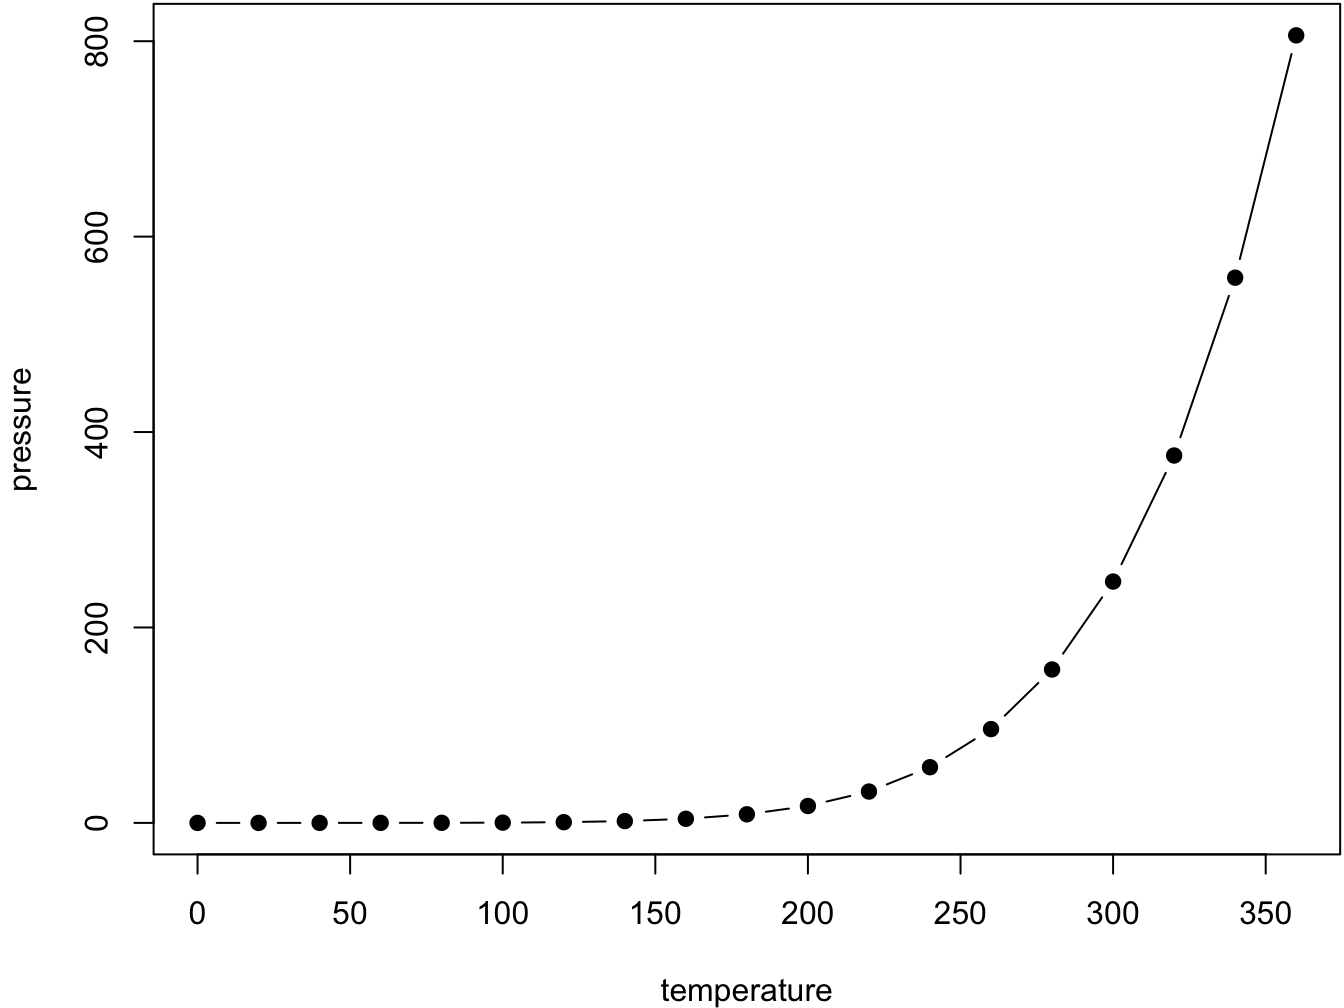
\includegraphics[width=0.8\linewidth]{me215projects_files/figure-latex/nice-fig-1} 

}

\caption{Here is a nice figure!}\label{fig:nice-fig}
\end{figure}

Reference a figure by its code chunk label with the \texttt{fig:} prefix, e.g., see Figure \ref{fig:nice-fig}. Similarly, you can reference tables generated from \texttt{knitr::kable()}, e.g., see Table \ref{tab:nice-tab}.

\begin{Shaded}
\begin{Highlighting}[]
\NormalTok{knitr}\OperatorTok{::}\KeywordTok{kable}\NormalTok{(}
  \KeywordTok{head}\NormalTok{(iris, }\DecValTok{20}\NormalTok{), }\DataTypeTok{caption =} \StringTok{\textquotesingle{}Here is a nice table!\textquotesingle{}}\NormalTok{,}
  \DataTypeTok{booktabs =} \OtherTok{TRUE}
\NormalTok{)}
\end{Highlighting}
\end{Shaded}

\begin{table}

\caption{\label{tab:nice-tab}Here is a nice table!}
\centering
\begin{tabular}[t]{rrrrl}
\toprule
Sepal.Length & Sepal.Width & Petal.Length & Petal.Width & Species\\
\midrule
5.1 & 3.5 & 1.4 & 0.2 & setosa\\
4.9 & 3.0 & 1.4 & 0.2 & setosa\\
4.7 & 3.2 & 1.3 & 0.2 & setosa\\
4.6 & 3.1 & 1.5 & 0.2 & setosa\\
5.0 & 3.6 & 1.4 & 0.2 & setosa\\
\addlinespace
5.4 & 3.9 & 1.7 & 0.4 & setosa\\
4.6 & 3.4 & 1.4 & 0.3 & setosa\\
5.0 & 3.4 & 1.5 & 0.2 & setosa\\
4.4 & 2.9 & 1.4 & 0.2 & setosa\\
4.9 & 3.1 & 1.5 & 0.1 & setosa\\
\addlinespace
5.4 & 3.7 & 1.5 & 0.2 & setosa\\
4.8 & 3.4 & 1.6 & 0.2 & setosa\\
4.8 & 3.0 & 1.4 & 0.1 & setosa\\
4.3 & 3.0 & 1.1 & 0.1 & setosa\\
5.8 & 4.0 & 1.2 & 0.2 & setosa\\
\addlinespace
5.7 & 4.4 & 1.5 & 0.4 & setosa\\
5.4 & 3.9 & 1.3 & 0.4 & setosa\\
5.1 & 3.5 & 1.4 & 0.3 & setosa\\
5.7 & 3.8 & 1.7 & 0.3 & setosa\\
5.1 & 3.8 & 1.5 & 0.3 & setosa\\
\bottomrule
\end{tabular}
\end{table}

You can write citations, too. For example, we are using the \textbf{bookdown} package \citep{R-bookdown} in this sample book, which was built on top of R Markdown and \textbf{knitr} \citep{xie2015}.

\hypertarget{literature}{%
\chapter{Literature}\label{literature}}

Here is a review of existing methods.

\hypertarget{quick-chill}{%
\chapter{Quick Chill}\label{quick-chill}}

\textbf{N05-164, US Navy Request for Proposals}

\emph{Technology areas}\\
Materials/Processes, Human Systems

\emph{Objective}\\
Develop an energy efficient, rugged, shipboard capability to quickly chill a canned beverage product (e.g., soda pop, or ``soft drink'') to help eliminate the requirement for operating traditional vending machines at sea.

\hypertarget{project-summary}{%
\section{Project Summary}\label{project-summary}}

For the primary customer on a ship (male, 22 years old), a key Quality of Life (QOL) element as documented by customer surveys is the ability to obtain a cold soft drink from a vending machine. That the per capita consumption of the commodity is almost double the U.S. per capita rate (52 gal a year) testifies to the popularity and desirability of this service. To satisfy this demand, the Navy as part of its QOL programs provides soft drink vending machines on ships. The design of the ship (storerooms separated from selling locations) coupled with the lack of transportation aids and the requirement to have up to 14 machines on larger ships has driven large platforms to devote up to six (6) man-years of effort to keep the machines filled. As the cost of manpower has increased, the need to find alternatives to provide this key QOL product has grown.

The desire is to develop a device capable of chilling a soft drink within 10 seconds, which is estimated to be the upper limit, or customer wait time tolerance, for the beverage consumer. The militarized version of the device needs to be compact and reliable, with little or no in-service maintenance requirements. Such a device, when distributed throughout the shipboard environment, could provide the following benefits:

\begin{enumerate}
\def\labelenumi{\arabic{enumi}.}
\tightlist
\item
  Eliminate, or minimize, shipboard requirements for environmentally threatening use of refrigerants (o-zone deleting substances)\\
\item
  Potentially remove all labor requirements involved in the operation of vending machines.\\
\item
  Removing the requirement for the product to be chilled at the point-of-sale, enabling more purchasing and storage flexibility to both the retailer (Ship's Store) and the consumer (sailor)
\end{enumerate}

\hypertarget{background}{%
\section{Background}\label{background}}

The rapid chilling of bulk food products (e.g., dairy, fruits \& vegetables) and especially solid food (e.g., carcass meat, fresh fish) is a long sought-after industry endeavor that has posted modest advances, with futuristic sights on a capability akin to a ``reverse microwave''. Restricted by the same heat transfer principles, the objective to rapidly chill a packaged consumer beverage can proceed towards a similar outcome when, and if, technology pushes past the decades-old capability of the vending machine. Rapid chill, with chill-on-demand service, is an evolutionary step away from the trappings of 20th century vending technology.

Consumer appeal for a chill on demand capability is demonstrated in sales of counter-top, household products promising to chill a bottle of wine in six minutes, or a canned beverage in one minute. However, products currently known to be available are extremely limited in applicability, essentially relegated to home use given the need to add both water and ice to the device. Other chill-on-demand technologies include a self-refrigerating beverage can promising to cool 30 °F in three minutes.

While these two examples of technological applications demonstrate the variability in potential approaches for obtaining the desired objective, neither is close to the required shipboard solution (ease-of-use, adequate chilling within 10 seconds). In addition, before any organization will embrace a modern technology, it will determine if the cost of new technology is ``affordable'' either in acquisition cost or ``tradeoff'' cost of providing the current service. The shipboard technical requirement exceeds any technology known to be available in the marketplace, and therefore presents unusually high technical risk. For these reasons, some leeway may be accommodated for the desired objective considering the proposed study approaches received.

\hypertarget{your-responsibilities}{%
\section{Your responsibilities}\label{your-responsibilities}}

Investigate alternative technologies/approaches to rapidly chill aluminum can packaged soft drinks/beverages. Evaluate and document alternatives and a developmental approach for one or more candidate devices.

A promising method is to have a chamber (or chambers) submerged in the drink. In the chamber is a fluid under pressure that will vaporize at atmospheric pressure and normal room temperature. When the chambers are opened, the fluid vaporizes. The Second Law demands the vaporization. The First Law demands the energy required for the phase change to take place. That energy is taken from anything in contact; it cannot be avoided. In this case, the energy is stolen from the soft drink, cooling it. \emph{Yes, this is what causes an aerosol can to get cold when sprayed.}

Other methods abound, but I'm less familiar with how they work. You're free to propose anything feasible. I'm willing to help you sort out your ideas as well.

\begin{enumerate}
\def\labelenumi{\arabic{enumi}.}
\tightlist
\item
  Develop a device capable of chilling a soft drink within 10 seconds.
\item
  Assume the soft drink is 12 fl.~oz. of water.\\
\item
  Assume the soft drink is initially 30,°C and must be chilled to 1,°C.
\item
  Use any of the substances tabulated in any textbook, ASHRAE manuals, or CoolProp.
\item
  Check for toxicity. I'm no advertising expert, but killing customers seems like it may potentially harm sales.
\end{enumerate}

\hypertarget{stuff}{%
\chapter{Stuff}\label{stuff}}

Hello, it's me. math 6 x 45 = 270. Did you know? maybe 8 * 9 = \texttt{julia\ 8*9}

\begin{Shaded}
\begin{Highlighting}[numbers=left,,firstnumber=100,]

\KeywordTok{using}\NormalTok{ Unitful      }\CommentTok{\# use unitful.jl units package for Julia}
\KeywordTok{using}\NormalTok{ Plots}

\NormalTok{V₂ }\OperatorTok{=}\NormalTok{ V₁ }\OperatorTok{*}\NormalTok{ (P₁}\OperatorTok{/}\NormalTok{P₂) }\OperatorTok{\^{}}\NormalTok{ (}\FloatTok{1}\OperatorTok{/}\NormalTok{n)    }\CommentTok{\# from eq(1)}
\NormalTok{𝑣₁ }\OperatorTok{=}\NormalTok{ V₁ }\OperatorTok{/}\NormalTok{ m                  }\CommentTok{\# from eq(2)}
\NormalTok{𝑣₂ }\OperatorTok{=}\NormalTok{ V₂ }\OperatorTok{/}\NormalTok{ m                  }\CommentTok{\# from eq(2)}
\NormalTok{println(}\StringTok{"V₂ = "}\OperatorTok{,}\NormalTok{V₂)}
\NormalTok{println(}\StringTok{"𝑣₁ = "}\OperatorTok{,}\NormalTok{𝑣₁)}
\NormalTok{println(}\StringTok{"𝑣₂ = "}\OperatorTok{,}\NormalTok{𝑣₂)}
\end{Highlighting}
\end{Shaded}

\begin{Shaded}
\begin{Highlighting}[]
\ExtensionTok{{-}{-}template}\NormalTok{=mda.html5, {-}{-}standalone, {-}{-}pdf{-}engine=xelatex, {-}{-}from=markdown+link\_attributes+fenced\_code\_blocks+backtick\_code\_blocks+fenced\_divs+fenced\_code\_attributes}
\end{Highlighting}
\end{Shaded}

\hypertarget{rocket-cryotanks}{%
\chapter{Rocket Cryotanks}\label{rocket-cryotanks}}

Here it is, finally, the replacemnt for Test One. There are two design problems described inside. Pick one. May 3 is the due date, but it's soft: if you need more time, let's discuss.

You may need property data beyond what is in your textbook. Feel free to use other texts, ASHRAE Handbooks, etc. Mathematica has a very nice thermodynamic properties function. The NIST\footnote{\citet{linstrom_nist_2019}} Chemistry WebBook may be a good option. Find it at \url{webbook.nist.gov}.

\hypertarget{coolprop}{%
\section{CoolProp}\label{coolprop}}

Perhaps the most straightforward access to thermodynamic properties is through CoolProp\footnote{\citet{bell_pure_2014}}, an open-source thermodynamic properties database.
I generally call CoolProp from within Julia or Python.
If you'd like to go that route, I can certainly help you get it all set up.
I can probably throw something together so you can use the same Jupyter Notebooks I use for problem solutions.

There is an online implementation of CoolProp where you can get properties one at a time, with no coding necessary.
Find it at\url{https://ibell.pythonanywhere.com}.
Here is the list of fluids available in CoolProp: \url{https://www.coolprop.org/fluid_properties/PurePseudoPure.html#list-of-fluids}.

\hypertarget{this-isnt-rocket-science}{%
\section{This isn't rocket science\ldots{}}\label{this-isnt-rocket-science}}

If you need help, or are feeling unsure, just ask. This assignment replaces Test One, but I do not intend for you to work on this alone. \textbf{Don't work with each other,} but ask me anything. Quite a bit of the physics involved transcend Thermodynamics I, and I suspect my simplifications won't cover every scenario you dream up.

\hypertarget{its-rocket-engineering}{%
\section{\ldots it's rocket engineering}\label{its-rocket-engineering}}

\begin{figure}

{\centering 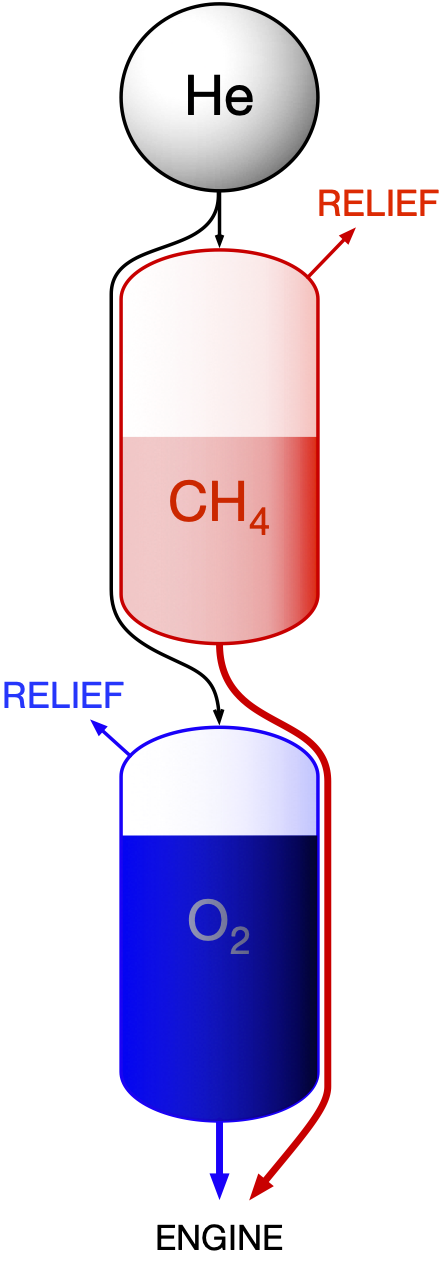
\includegraphics[width=0.25\linewidth]{./figures/rocket-fuel} 

}

\caption{Simple depiction of a rocket fuel system}\label{fig:rocket-fuel}
\end{figure}

Storing Cryogenic liquids is a challenging endeavor.
Cryogenic liquids have boiling points that are far below ambient temperature.
When storing them, a major challenge is reducing boil-off.
The cryogen is under saturation conditions.
Any heat transfer into the tank causes some of the cryogen to boil away, a serious concern for applications that requires liquid cryogen (as opposed to very cold gas).

Consider a rocket fueled by liquid methane (LMG), with liquid oxygen (LOX) oxidizer.
You are charged with designing the fuel system.
We've already determined how much fuel and oxidizer are required to complete the mission. Your major concern is the loss of LMG and LOX while the rocket sits on the pad. You will be launching from the New Mexico desert in mid-June, and the rocket may sit on the pad for up to 2 hours after fueling.
Because you're so good at thermodynamics, you know you have several options at your disposal:

\begin{enumerate}
\def\labelenumi{\arabic{enumi}.}
\tightlist
\item
  Increase tank pressure.
\item
  Insulate the tanks.
\item
  Load extra cryogens.
\end{enumerate}

\hypertarget{your-responsibilities}{%
\section{Your responsibilities}\label{your-responsibilities}}

\begin{enumerate}
\def\labelenumi{\arabic{enumi}.}
\tightlist
\item
  Size both tanks.
\item
  Specify the initial masses of LOX and LMG to be loaded into each tank. This is the amount before any boiloff begins.
\item
  Specify operating pressure of each tank.
\item
  Specify the insulation and its thickness.
\end{enumerate}

\hypertarget{constraints-and-requirements}{%
\section{Constraints and requirements}\label{constraints-and-requirements}}

\begin{enumerate}
\def\labelenumi{\arabic{enumi}.}
\tightlist
\item
  The time between loading and launch is 2 hours.
\item
  The outer wall skin temperature T\textsubscript{w} = 60,°C.
\item
  The inner wall skin temperature T\textsubscript{s} = T\textsubscript{sat} for the fluid, at the operating pressure you specify.
\item
  A minimum of 59 kg LMG and 235 kg LOX must be present at launch.
\item
  Assume the tanks are cylinders (flat top/bottom) with inner diameter D = 45 cm.
\item
  Each tank has a maximaum allowable working pressure of 2 bar.
\item
  Neither tank can contain \textgreater{} 80\% liquid, by volume.
\item
  A maximum of 4 inches is available between the tank outer wall and the rocket inner wall.
\item
  It's a rocket. Low weight is holy and just.
\end{enumerate}

\hypertarget{heat-transfer}{%
\section{Heat Transfer}\label{heat-transfer}}

\noindent
In our case, we will simplify the heat transfer portion to basic conduction. Assume heat transfer into the tanks can be expressed as

\begin{equation}
 \dot Q_{in} = \frac{T_s - T_w}{R}
\end{equation}

where

\begin{gather*}
  \begin{split}
    T_s &\equiv \text{outer wall skin temperature} \\
    T_w &\equiv \text{inner wall skin temperature} = T_{sat} \\
    R &\equiv   \text{thermal resistance} = \frac{L}{kA} 
  \end{split} \\
 \qquad
  \begin{split}
   L & \equiv \text{insulation thickness} \\
   k & \equiv \text{insulation thermal conductivity} \\
   A & \equiv \text{tank surface area} \\
  \end{split} \\ {}
\end{gather*}

Thermal resistance \emph{R} is \emph{sometimes} the R-value you see on insulation packaging, but the units are rarely given on the product label.
However, you can usually find the thermal conductivity \emph{k} in datasheets at the manufacturers website.
Table A19 in your text lists thermal conductivity for many common materials.
You might be interested in Aerogel, an extreme performance insulation, where
\(k = 0.023\, W/m \cdot K\).
I will help you find \emph{k} (or any values) if you ask.

\hypertarget{methods}{%
\chapter{Methods}\label{methods}}

We describe our methods in this chapter.

\hypertarget{applications}{%
\chapter{Applications}\label{applications}}

Some \emph{significant} applications are demonstrated in this chapter.

\hypertarget{example-one}{%
\section{Example one}\label{example-one}}

\hypertarget{example-two}{%
\section{Example two}\label{example-two}}

\hypertarget{final-words}{%
\chapter{Final Words}\label{final-words}}

We have finished a nice book.

  \bibliography{book.bib,packages.bib}

\end{document}
